% Graphic for TeX using PGF
% Title: /home/braulio/Git/TFG/clases.dia
% Creator: Dia v0.97.3
% CreationDate: Mon Oct 24 17:22:42 2016
% For: braulio
% \usepackage{tikz}
% The following commands are not supported in PSTricks at present
% We define them conditionally, so when they are implemented,
% this pgf file will use them.
\ifx\du\undefined
  \newlength{\du}
\fi
\setlength{\du}{15\unitlength}
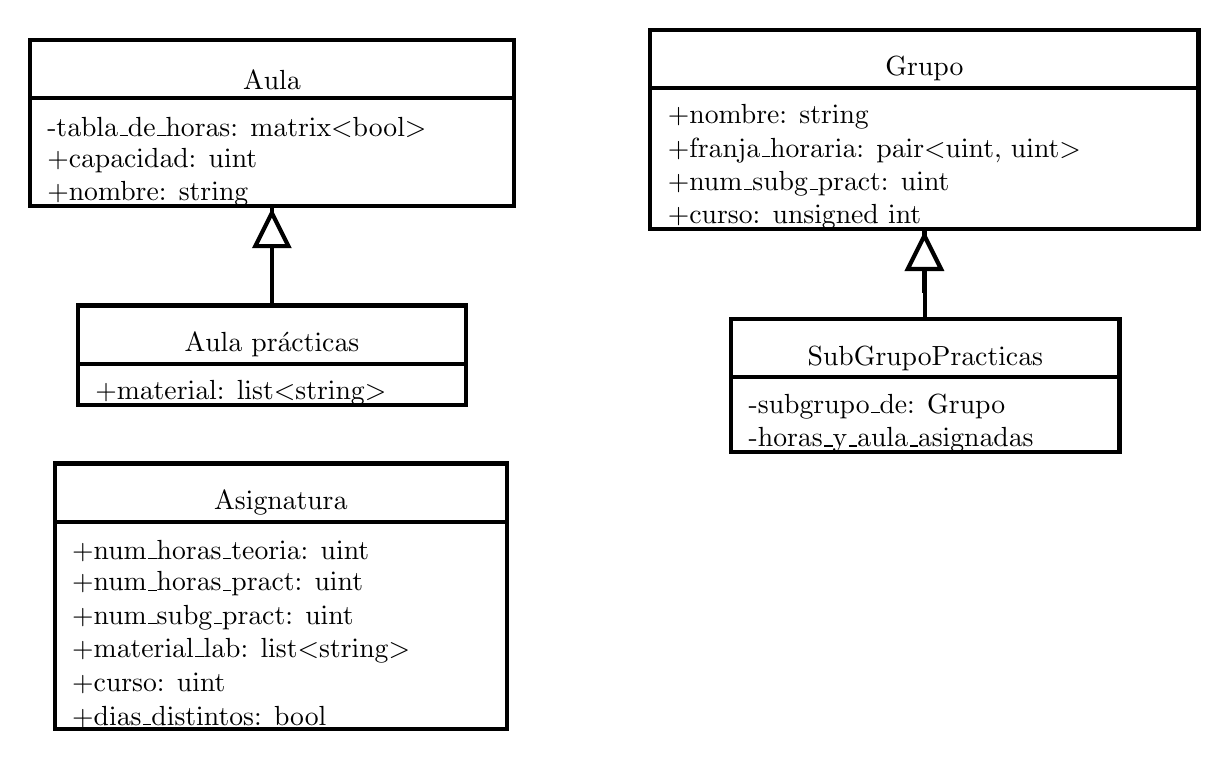
\begin{tikzpicture}
\pgftransformxscale{1.000000}
\pgftransformyscale{-1.000000}
\definecolor{dialinecolor}{rgb}{0.000000, 0.000000, 0.000000}
\pgfsetstrokecolor{dialinecolor}
\definecolor{dialinecolor}{rgb}{1.000000, 1.000000, 1.000000}
\pgfsetfillcolor{dialinecolor}
\pgfsetlinewidth{0.100000\du}
\pgfsetdash{}{0pt}
\definecolor{dialinecolor}{rgb}{1.000000, 1.000000, 1.000000}
\pgfsetfillcolor{dialinecolor}
\fill (11.650000\du,5.000000\du)--(11.650000\du,6.400000\du)--(23.315000\du,6.400000\du)--(23.315000\du,5.000000\du)--cycle;
\definecolor{dialinecolor}{rgb}{0.000000, 0.000000, 0.000000}
\pgfsetstrokecolor{dialinecolor}
\draw (11.650000\du,5.000000\du)--(11.650000\du,6.400000\du)--(23.315000\du,6.400000\du)--(23.315000\du,5.000000\du)--cycle;
% setfont left to latex
\definecolor{dialinecolor}{rgb}{0.000000, 0.000000, 0.000000}
\pgfsetstrokecolor{dialinecolor}
\node at (17.482500\du,5.950000\du){Aula};
\definecolor{dialinecolor}{rgb}{1.000000, 1.000000, 1.000000}
\pgfsetfillcolor{dialinecolor}
\fill (11.650000\du,6.400000\du)--(11.650000\du,9.000000\du)--(23.315000\du,9.000000\du)--(23.315000\du,6.400000\du)--cycle;
\definecolor{dialinecolor}{rgb}{0.000000, 0.000000, 0.000000}
\pgfsetstrokecolor{dialinecolor}
\draw (11.650000\du,6.400000\du)--(11.650000\du,9.000000\du)--(23.315000\du,9.000000\du)--(23.315000\du,6.400000\du)--cycle;
% setfont left to latex
\definecolor{dialinecolor}{rgb}{0.000000, 0.000000, 0.000000}
\pgfsetstrokecolor{dialinecolor}
\node[anchor=west] at (11.800000\du,7.100000\du){-tabla\_de\_horas: matrix$<$bool$>$};
% setfont left to latex
\definecolor{dialinecolor}{rgb}{0.000000, 0.000000, 0.000000}
\pgfsetstrokecolor{dialinecolor}
\node[anchor=west] at (11.800000\du,7.900000\du){+capacidad: uint};
% setfont left to latex
\definecolor{dialinecolor}{rgb}{0.000000, 0.000000, 0.000000}
\pgfsetstrokecolor{dialinecolor}
\node[anchor=west] at (11.800000\du,8.700000\du){+nombre: string};
\pgfsetlinewidth{0.100000\du}
\pgfsetdash{}{0pt}
\definecolor{dialinecolor}{rgb}{1.000000, 1.000000, 1.000000}
\pgfsetfillcolor{dialinecolor}
\fill (12.806645\du,11.392000\du)--(12.806645\du,12.792000\du)--(22.161645\du,12.792000\du)--(22.161645\du,11.392000\du)--cycle;
\definecolor{dialinecolor}{rgb}{0.000000, 0.000000, 0.000000}
\pgfsetstrokecolor{dialinecolor}
\draw (12.806645\du,11.392000\du)--(12.806645\du,12.792000\du)--(22.161645\du,12.792000\du)--(22.161645\du,11.392000\du)--cycle;
% setfont left to latex
\definecolor{dialinecolor}{rgb}{0.000000, 0.000000, 0.000000}
\pgfsetstrokecolor{dialinecolor}
\node at (17.484145\du,12.342000\du){Aula prácticas};
\definecolor{dialinecolor}{rgb}{1.000000, 1.000000, 1.000000}
\pgfsetfillcolor{dialinecolor}
\fill (12.806645\du,12.792000\du)--(12.806645\du,13.792000\du)--(22.161645\du,13.792000\du)--(22.161645\du,12.792000\du)--cycle;
\definecolor{dialinecolor}{rgb}{0.000000, 0.000000, 0.000000}
\pgfsetstrokecolor{dialinecolor}
\draw (12.806645\du,12.792000\du)--(12.806645\du,13.792000\du)--(22.161645\du,13.792000\du)--(22.161645\du,12.792000\du)--cycle;
% setfont left to latex
\definecolor{dialinecolor}{rgb}{0.000000, 0.000000, 0.000000}
\pgfsetstrokecolor{dialinecolor}
\node[anchor=west] at (12.956645\du,13.492000\du){+material: list$<$string$>$};
\pgfsetlinewidth{0.100000\du}
\pgfsetdash{}{0pt}
\pgfsetmiterjoin
\pgfsetbuttcap
{
\definecolor{dialinecolor}{rgb}{0.000000, 0.000000, 0.000000}
\pgfsetfillcolor{dialinecolor}
% was here!!!
\definecolor{dialinecolor}{rgb}{0.000000, 0.000000, 0.000000}
\pgfsetstrokecolor{dialinecolor}
\draw (17.482500\du,9.050250\du)--(17.482500\du,10.595973\du)--(17.484145\du,10.595973\du)--(17.484145\du,11.341695\du);
}
\definecolor{dialinecolor}{rgb}{0.000000, 0.000000, 0.000000}
\pgfsetstrokecolor{dialinecolor}
\draw (17.482500\du,9.962054\du)--(17.482500\du,10.595973\du)--(17.484145\du,10.595973\du)--(17.484145\du,11.341695\du);
\pgfsetmiterjoin
\definecolor{dialinecolor}{rgb}{1.000000, 1.000000, 1.000000}
\pgfsetfillcolor{dialinecolor}
\fill (17.882500\du,9.962054\du)--(17.482500\du,9.162054\du)--(17.082500\du,9.962054\du)--cycle;
\pgfsetlinewidth{0.100000\du}
\pgfsetdash{}{0pt}
\pgfsetmiterjoin
\definecolor{dialinecolor}{rgb}{0.000000, 0.000000, 0.000000}
\pgfsetstrokecolor{dialinecolor}
\draw (17.882500\du,9.962054\du)--(17.482500\du,9.162054\du)--(17.082500\du,9.962054\du)--cycle;
% setfont left to latex
\pgfsetlinewidth{0.100000\du}
\pgfsetdash{}{0pt}
\definecolor{dialinecolor}{rgb}{1.000000, 1.000000, 1.000000}
\pgfsetfillcolor{dialinecolor}
\fill (26.600000\du,4.750000\du)--(26.600000\du,6.150000\du)--(39.805000\du,6.150000\du)--(39.805000\du,4.750000\du)--cycle;
\definecolor{dialinecolor}{rgb}{0.000000, 0.000000, 0.000000}
\pgfsetstrokecolor{dialinecolor}
\draw (26.600000\du,4.750000\du)--(26.600000\du,6.150000\du)--(39.805000\du,6.150000\du)--(39.805000\du,4.750000\du)--cycle;
% setfont left to latex
\definecolor{dialinecolor}{rgb}{0.000000, 0.000000, 0.000000}
\pgfsetstrokecolor{dialinecolor}
\node at (33.202500\du,5.700000\du){Grupo};
\definecolor{dialinecolor}{rgb}{1.000000, 1.000000, 1.000000}
\pgfsetfillcolor{dialinecolor}
\fill (26.600000\du,6.150000\du)--(26.600000\du,9.550000\du)--(39.805000\du,9.550000\du)--(39.805000\du,6.150000\du)--cycle;
\definecolor{dialinecolor}{rgb}{0.000000, 0.000000, 0.000000}
\pgfsetstrokecolor{dialinecolor}
\draw (26.600000\du,6.150000\du)--(26.600000\du,9.550000\du)--(39.805000\du,9.550000\du)--(39.805000\du,6.150000\du)--cycle;
% setfont left to latex
\definecolor{dialinecolor}{rgb}{0.000000, 0.000000, 0.000000}
\pgfsetstrokecolor{dialinecolor}
\node[anchor=west] at (26.750000\du,6.850000\du){+nombre: string};
% setfont left to latex
\definecolor{dialinecolor}{rgb}{0.000000, 0.000000, 0.000000}
\pgfsetstrokecolor{dialinecolor}
\node[anchor=west] at (26.750000\du,7.650000\du){+franja\_horaria: pair$<$uint, uint$>$};
% setfont left to latex
\definecolor{dialinecolor}{rgb}{0.000000, 0.000000, 0.000000}
\pgfsetstrokecolor{dialinecolor}
\node[anchor=west] at (26.750000\du,8.450000\du){+num\_subg\_pract: uint};
% setfont left to latex
\definecolor{dialinecolor}{rgb}{0.000000, 0.000000, 0.000000}
\pgfsetstrokecolor{dialinecolor}
\node[anchor=west] at (26.750000\du,9.250000\du){+curso: unsigned int};
\pgfsetlinewidth{0.100000\du}
\pgfsetdash{}{0pt}
\definecolor{dialinecolor}{rgb}{1.000000, 1.000000, 1.000000}
\pgfsetfillcolor{dialinecolor}
\fill (12.250000\du,15.200000\du)--(12.250000\du,16.600000\du)--(23.145000\du,16.600000\du)--(23.145000\du,15.200000\du)--cycle;
\definecolor{dialinecolor}{rgb}{0.000000, 0.000000, 0.000000}
\pgfsetstrokecolor{dialinecolor}
\draw (12.250000\du,15.200000\du)--(12.250000\du,16.600000\du)--(23.145000\du,16.600000\du)--(23.145000\du,15.200000\du)--cycle;
% setfont left to latex
\definecolor{dialinecolor}{rgb}{0.000000, 0.000000, 0.000000}
\pgfsetstrokecolor{dialinecolor}
\node at (17.697500\du,16.150000\du){Asignatura};
\definecolor{dialinecolor}{rgb}{1.000000, 1.000000, 1.000000}
\pgfsetfillcolor{dialinecolor}
\fill (12.250000\du,16.600000\du)--(12.250000\du,21.600000\du)--(23.145000\du,21.600000\du)--(23.145000\du,16.600000\du)--cycle;
\definecolor{dialinecolor}{rgb}{0.000000, 0.000000, 0.000000}
\pgfsetstrokecolor{dialinecolor}
\draw (12.250000\du,16.600000\du)--(12.250000\du,21.600000\du)--(23.145000\du,21.600000\du)--(23.145000\du,16.600000\du)--cycle;
% setfont left to latex
\definecolor{dialinecolor}{rgb}{0.000000, 0.000000, 0.000000}
\pgfsetstrokecolor{dialinecolor}
\node[anchor=west] at (12.400000\du,17.300000\du){+num\_horas\_teoria: uint};
% setfont left to latex
\definecolor{dialinecolor}{rgb}{0.000000, 0.000000, 0.000000}
\pgfsetstrokecolor{dialinecolor}
\node[anchor=west] at (12.400000\du,18.100000\du){+num\_horas\_pract: uint};
% setfont left to latex
\definecolor{dialinecolor}{rgb}{0.000000, 0.000000, 0.000000}
\pgfsetstrokecolor{dialinecolor}
\node[anchor=west] at (12.400000\du,18.900000\du){+num\_subg\_pract: uint};
% setfont left to latex
\definecolor{dialinecolor}{rgb}{0.000000, 0.000000, 0.000000}
\pgfsetstrokecolor{dialinecolor}
\node[anchor=west] at (12.400000\du,19.700000\du){+material\_lab: list$<$string$>$};
% setfont left to latex
\definecolor{dialinecolor}{rgb}{0.000000, 0.000000, 0.000000}
\pgfsetstrokecolor{dialinecolor}
\node[anchor=west] at (12.400000\du,20.500000\du){+curso: uint};
% setfont left to latex
\definecolor{dialinecolor}{rgb}{0.000000, 0.000000, 0.000000}
\pgfsetstrokecolor{dialinecolor}
\node[anchor=west] at (12.400000\du,21.300000\du){+dias\_distintos: bool};
\pgfsetlinewidth{0.100000\du}
\pgfsetdash{}{0pt}
\definecolor{dialinecolor}{rgb}{1.000000, 1.000000, 1.000000}
\pgfsetfillcolor{dialinecolor}
\fill (28.547045\du,11.725000\du)--(28.547045\du,13.125000\du)--(37.902045\du,13.125000\du)--(37.902045\du,11.725000\du)--cycle;
\definecolor{dialinecolor}{rgb}{0.000000, 0.000000, 0.000000}
\pgfsetstrokecolor{dialinecolor}
\draw (28.547045\du,11.725000\du)--(28.547045\du,13.125000\du)--(37.902045\du,13.125000\du)--(37.902045\du,11.725000\du)--cycle;
% setfont left to latex
\definecolor{dialinecolor}{rgb}{0.000000, 0.000000, 0.000000}
\pgfsetstrokecolor{dialinecolor}
\node at (33.224545\du,12.675000\du){SubGrupoPracticas};
\definecolor{dialinecolor}{rgb}{1.000000, 1.000000, 1.000000}
\pgfsetfillcolor{dialinecolor}
\fill (28.547045\du,13.125000\du)--(28.547045\du,14.925000\du)--(37.902045\du,14.925000\du)--(37.902045\du,13.125000\du)--cycle;
\definecolor{dialinecolor}{rgb}{0.000000, 0.000000, 0.000000}
\pgfsetstrokecolor{dialinecolor}
\draw (28.547045\du,13.125000\du)--(28.547045\du,14.925000\du)--(37.902045\du,14.925000\du)--(37.902045\du,13.125000\du)--cycle;
% setfont left to latex
\definecolor{dialinecolor}{rgb}{0.000000, 0.000000, 0.000000}
\pgfsetstrokecolor{dialinecolor}
\node[anchor=west] at (28.697045\du,13.825000\du){-subgrupo\_de: Grupo};
% setfont left to latex
\definecolor{dialinecolor}{rgb}{0.000000, 0.000000, 0.000000}
\pgfsetstrokecolor{dialinecolor}
\node[anchor=west] at (28.697045\du,14.625000\du){-horas\_y\_aula\_asignadas};
\pgfsetlinewidth{0.100000\du}
\pgfsetdash{}{0pt}
\pgfsetmiterjoin
\pgfsetbuttcap
{
\definecolor{dialinecolor}{rgb}{0.000000, 0.000000, 0.000000}
\pgfsetfillcolor{dialinecolor}
% was here!!!
\definecolor{dialinecolor}{rgb}{0.000000, 0.000000, 0.000000}
\pgfsetstrokecolor{dialinecolor}
\draw (33.202500\du,9.600299\du)--(33.202500\du,11.037448\du)--(33.224545\du,11.037448\du)--(33.224545\du,11.674597\du);
}
\definecolor{dialinecolor}{rgb}{0.000000, 0.000000, 0.000000}
\pgfsetstrokecolor{dialinecolor}
\draw (33.202500\du,10.512102\du)--(33.202500\du,11.037448\du)--(33.224545\du,11.037448\du)--(33.224545\du,11.674597\du);
\pgfsetmiterjoin
\definecolor{dialinecolor}{rgb}{1.000000, 1.000000, 1.000000}
\pgfsetfillcolor{dialinecolor}
\fill (33.602500\du,10.512102\du)--(33.202500\du,9.712102\du)--(32.802500\du,10.512102\du)--cycle;
\pgfsetlinewidth{0.100000\du}
\pgfsetdash{}{0pt}
\pgfsetmiterjoin
\definecolor{dialinecolor}{rgb}{0.000000, 0.000000, 0.000000}
\pgfsetstrokecolor{dialinecolor}
\draw (33.602500\du,10.512102\du)--(33.202500\du,9.712102\du)--(32.802500\du,10.512102\du)--cycle;
% setfont left to latex
\end{tikzpicture}
